\section*{Введение}

В жизненном цикле программного обеспечения важную роль занимает этап
поддержки [здесь ссылка на статью De Marco?]. Этот этап по разным оценкам
составляет от 30 до 60\% общего бюджета проекта. Поэтому для
промышленного программного кода важно, чтобы его было легко читать и изменять.
Рассмотрим описание функций
на рисунках~\ref{fig:wikiExUnfor} и \ref{fig:wikiExBSD}.

\begin{figure}[h!]
	\centering
	\lstinputlisting[language=C]{codes/wikiExUnfor.c}
	\caption{Неформатированный код}
	\label{fig:wikiExUnfor}
\end{figure}

\begin{figure}[h!]
	\centering
	\lstinputlisting[language=C]{codes/wikiExBSD.c}
  \caption{Форматированный код (BSD)}
	\label{fig:wikiExBSD}
\end{figure}

Эти функции семантически и синтаксически эквиваленты с точки зрения
компилятора C, но вариант, приведенный на
рисунке~\ref{fig:wikiExUnfor}, гораздо хуже
поддается понимаю человека и требует большего времени на изменение,
что увеличивает стоимость и трудозатраты на поддержку. Как мы видим из этого
примера, программные тексты должны явным образом отражать
структуру синтаксического дерева программы.

Кроме того, распространенной практикой [ссылка на статью про стандарты
кодирования], доказавшей свою состоятельность, является использования
общепроектного стандарта кодирования (\textit{coding convention}).
\textbf{Стандарт кодирования (СК)} ---
это набор соглашений, которые используются
при написании программного кода. В него входят: способы выбора имен переменных
и других идентификаторов, стили отступов при оформлении логических блоков,
способы расстановки ограничителей логических блоков (скобок),
форматы комментариев. СК также призван упростить анализ и изменение
программы, поэтому его важно соблюдать, что вводит
дополнительные ограничения на исходные тексты. СК разных проектов, даже
реализуемых на одном и том же языке программирования, могут существенно
различаться.
Так код на рисунке~\ref{fig:wikiExBSD} соответствует СК BSD,
а на рисунке~\ref{fig:wikiExGNU} --- GNU.

\begin{figure}[h!]
	\centering
	\lstinputlisting[language=C]{codes/wikiExGNU.c}
  \caption{Форматированный код (GNU)}
	\label{fig:wikiExGNU}
\end{figure}

Кроме ситуаций, когда СК в проекте поддерживается при ручном написании
программного кода, существует другой важный пример использования СК ---
в языковых процессорах. \textbf{Языковой процессор} (\textbf{ЯП}) ---
это программное средство, принимающее на вход программу в виде текста
на некотором языке (программирования, разметки и т. д.) и решающее
определенную задачу над этой программой. К языковым процессорам можно
отнести: компиляторы, суперкомпиляторы, интерпретаторы,
средства статического анализа кода, декомпиляторы, средства рефакторинга,
средства реинжиниринга, интегрированные среды разработки (IDE) и др.

Первым этапом работы ЯП является \textbf{синтаксический анализ}, то есть
сопоставление входного текста (линейной последовательности лексем) с формальной
грамматикой языка. В результате работы синтаксического анализатора ЯП получает
древовидное представление программы, над которым потом происходит основная работа.

Дальше перед большим классом ЯП возникает задача показать пользователю
промежуточный или конечный результат обработки кода.
Следовательно, необходимо вернуться к текстовому представлению программы,
то есть провести процедуру, обратную синтаксическому анализу. Такая задача
называется \textbf{pretty printing}, а соответствующий инструмент ---
\textbf{pretty printer}. Далее этот инструмент мы будем называть
\textbf{принтером}.

Сформулируем требования, которые накладываются на принтер.
Как уже понятно, принтер должен
продуцировать текст, который удовлетворяет проектому СК в части
форматирования логических структур и отступов.
Это ограничение также должно решать проблему наглядности кода в том смысле,
что в тексте явным образом отражается логическая структура программы.
В большинстве случаев СК оставляет некоторую свободу в представлении
синтаксической конструкции и тогда осмысленно вводить дополнительное
ограничение на ширину вывода принтера, а среди подходящих представлений
искать \textit{оптимальное}. Часто в данном случае под
оптимальным вариантом представления понимают тот вариант,
что занимает минимальное число строчек,
то есть улучшает свойство \textit{обозримости} текста.

С другой стороны, понятие принтера можно формализовать как функцию,
которая на вход принимает
абстрактное или конкрентное синтаксическое дерево и дополнительные параметры,
а на выходе выдает текст. В случае, если на вход принтеру подается конкретное
синтаксическое дерево, то есть дерево разбора, принтер может быть частичной
функцией по отношению к синтаксическим конструкциям языка.
Такое ослабление связано
с тем, что для конструкций, на которых принтер не определен, можно использовать
их текстовое представление, заложенное в дерево разбора.   

Рассмотрим небольшой пример.
Пусть в СК задано условие вида: “последовательные операторы пишутся
на одной строке,
если помещаются в N символов, а иначе --- на разных строках”.

\begin{figure}[h!]
	\centering
	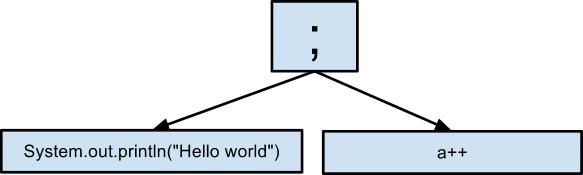
\includegraphics[width=0.8\textwidth]{seqTree}
	\caption{Последовательные операторы}
	\label{fig:seqImage}
\end{figure}

На рисунке~\ref{fig:seqImage} изображено синтаксическое дерево
последовательности двух операторов. Такое дерево, согласно заданному
правилу, может быть напечатано одним из
двух вариантов (рисунки ~\ref{fig:seqCode1}, ~\ref{fig:seqCode2}).

\begin{figure}[h!]
	\centering
	% \inputminted{c}{codes/seqCode1.java}
	\lstinputlisting[language=Java]{codes/seqCode1.java}
	\caption{Последовательные операторы в строчку}
	\label{fig:seqCode1}
\end{figure}

\begin{figure}[h!]
	\centering
	% \inputminted{c}{codes/seqCode2.java}
	\lstinputlisting[language=Java]{codes/seqCode2.java}
	\caption{Последовательные операторы в несколько строк}
	\label{fig:seqCode2}
\end{figure}

Выбор происходит в зависимости от ширины вывода. Так, при ширине равной
35 символов (длина строки <<System.out.println(“Hello world”); >>),
должен выбираться вариант, изображенный на рисунке~\ref{fig:seqCode2},
так как код на рисунке~\ref{fig:seqCode1} имеет ширину более 35 символов.
Могут быть заданы и более сложные условия.

Рассмотрим другой пример.
Пусть нам нужно текстовое представление синтаксического дерева конструкции
“\lstinline{if}”, и заданы шаблоны c рисунков~\ref{fig:ifTemplate2} и
\ref{fig:ifTemplate1}. При этом вариант, изображенный на
рисунке~\ref{fig:ifTemplate2} выбирается только в случае, если условие и
ветки могут быть напечатаны в одну строчку.

\begin{figure}[h!]
	\subfloat[]{
		\lstinputlisting[language=Haskell]{codes/ifTemplate2.hs}
		\label{fig:ifTemplate2}	
	}
	\quad
	\subfloat[]{
		\lstinputlisting[language=Haskell]{codes/ifTemplate1.hs}
		\label{fig:ifTemplate1}	
	}
	\caption{Представления для конструкции “\lstinline{if}”}
\end{figure}


Тогда для деревьев, представленных на рисунках
\ref{fig:ifImage1} и \ref{fig:ifImage2}, будут напечатаны коды с
рисунков \ref{fig:ifCode1} и \ref{fig:ifCode2} соответственно.

\begin{figure}[h!]
	\subfloat[]{
		\centering
		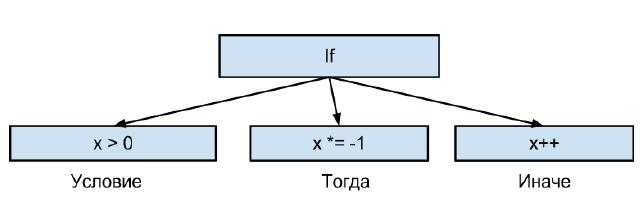
\includegraphics[width=0.6\textwidth]{if1}
		\label{fig:ifImage1}
	}
	\quad
	\subfloat[]{
		\centering
		% \inputminted{haskell}{codes/ifCode1.hs}
		\lstinputlisting[language=Haskell]{codes/ifCode1.hs}
		\label{fig:ifCode1}	
	}

	\caption{Использование представления с рис.~\ref{fig:ifTemplate2}}
\end{figure}

\begin{figure}[h!]
	\subfloat[]{
		\centering
		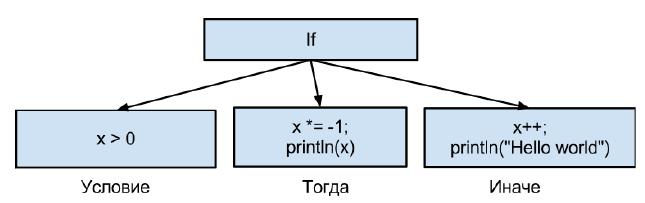
\includegraphics[width=0.6\textwidth]{if2}
		\label{fig:ifImage2}
	}
	\quad
	\subfloat[]{
		\centering
		% \inputminted{haskell}{codes/ifCode1.hs}
		\lstinputlisting[language=Haskell]{codes/ifCode2.hs}
		\label{fig:ifCode2}	
	}

	\caption{Использование представления с рис.~\ref{fig:ifTemplate1}}
\end{figure}

\subsection{In work}

Существует несколько методик написания принтеров. 
Классическим способом задания принтеров в функциональных языках
программирования являются
принтер-комбинаторы~\cite{wadler, swierstra, swierstraChitil,
swierstra04, hughes, peytonJones, kiselyov, chitil, swiComb}.

Кроме того, есть работы посвященные получению принтера по синтаксическому
анализатору и наоборот~\cite{rendelInvert}.
Они вводят отношение \textit{частичного изоморфизма} на множествах абстрактных
и конкретных синтаксических деревьев. Введение такого отношения позволяет
совместно разрабатывать принтер и синтаксический анализатор. Кроме того,
что таким образом уменьшается общий объем работы, подобный подход позволяет
избежать несоответствия между принтером и анализатором.
С другой стороны, если необходимо иметь анализаторы и принтеры для нескольких
конкретных синтаксисов языка, при чем не для каждого синтаксиса надо иметь
и принтер, и анализатор, то разработка усложняется.

% Вообще-то под \textbf{комбинатором} понимается
% $\lambda$-терм без свободных переменных, но в нашем контексте о нем можно
% думать несколько проще --- как о функции высшего порядка,
% которая позволяет комбинировать сложный принтер из более простых.

В рамках предыдущей работы автора \cite{myCoursePaper} был разработан принтер
для учебного языка L, который использовал синтаксическое расширение парсера.
Это еще один пример того, как задачи решаются вместе.

\subsection{Постановка задачи}

% TODO
TODO

Целью данной работы является разработка метода задания принтеров с помощью
образцов для языков программирования. 
Для апробирования метода было принято решение разработать принтер-плагин
языка Java для среды разработки IntelliJ IDEA.
В ходе разработки данного метода возникла необходимость улучшить существующую
принтер-комбинаторную библиотеку\cite{swierstra}. 
